\chapter{Irodalmi áttekintés}
\section{Ipari ütemezési feladatok}
Az ipari folyamatok közé tartozó tevékenységeknek egy jelentős halmazát gyártásnak nevezzük, amely során az elkészítendő termék létrehozása, megvalósítása a feladat.
Ehhez szükség van arra, hogy megfelelően vegyük igénybe a rendelkezésre álló erőforrásokat, amelyeket berendezéseknek, unitnak nevezünk a gyártási feladatok során.
A folyamat során fellépő feladatokra a taszk elnevezés is használható.
Az ütemezés az a folyamat, amely során különböző események sorrendjét határozzuk meg.
Az ütemezési feladat során kell egy feladatot, munkát vagy tevékenységet egy tervbe beilleszteni, vagyis meghatározni annak végrehajtási időpontját.
Minden ütemezési feladat rendelkezik végrehajtási idővel, ami megmutatja mekkora időtartam alatt valósítható meg.
Ezenfelül lehet még a feladatoknak olyan időkorlátja, ami alatt kötelező elvégezni a feladatot, ezt időhorizontnak, time horizontnak hívjuk.
A problémák kimenetelük szerint lehetnek megvalósíthatatlan (infeasible) és megvalósítható (feasible) feladatok.
Egy feladat csak abban az esetben minősül megvalósíthatónak, ha minden korlátozásnak megfelel.
Ha már akár csak egy korlátozással szemben nem bizonyul elfogadhatónak, akkor infeasible feladatról beszélhetünk.

Az ipari folyamatokat többféleképpen lehet csoportosítani.
Az egyik felosztási módszer szerint folyamatos és szakaszos üzemű rendszerek csoportjára bontjuk őket.
Az első típusban az anyag folyamatosan kerül a rendszerbe, a másodikban pedig ez a folyamat lépésekben valósul meg.
A munkám az utóbbi típusba tartozó feladatokra koncentrál.
Másik lehetséges felosztás az, amikor online, offline, és semi-offline kategóriákba vannak a feladatok besorolva.
Az offline esetben minden szükséges bemeneti adat rendelkezésre áll az optimalizálás idejében.
Ezzel szemben az online esetben előbb kell a döntéseket meghozni, minthogy az adott paraméterekhez tartozó értékekre fény derülne.
A semi-offline a kettő közé sorolható, azaz bizonyos információk, adatok már rendelkezésre állnak, mások viszont nem.

Az ütemezési feladatok modelljét receptnek nevezzük.
Egy termék receptje tartalmazza az adott recept által előállítható termék elkészítéséhez szükséges információkat\cite{Hegyhati}.
Egy receptet a következő elemek közösen alkotják:
\begin{itemize}
  \item termékek listája,
  \item taszkok listája, amelyek adott sorrendben történő elvégzése szükséges a termék előállításához,
  \item termeléshez kapcsolódó taszkok sorrendje,
  \item rendelkezésre álló berendezések,
  \item a lehetséges taszk-berendezés párokhoz tartozó feldolgozási idő.
\end{itemize}

A recepteket a feladatok precedenciája szerint az alábbi csoportokba lehet besorolni.
A felsorolás a legegyszerűbbtől halad az általánosabb felé.
Minden osztály a következőnek egy speciális esete.
\begin{itemize}
	\item \textbf{Single Stage:} Egy lépésben állítható elő minden egyes termék.
	\item \textbf{Simple Multiproduct:} Minden terméket meghatározott számú fázison, szakaszon keresztül lehet elkészíteni.
	Előzővel szemben itt már nem csak egy lépésben lehetséges.
	Különösen fontos, hogy nem lehet elágazás benne, azaz csak szekvenciális lehet.
	\item \textbf{General Multiproduct:} Előzővel összehasonlítva az a különbség, hogy ennél lehetséges lépések kihagyása.
	\item \textbf{Multipurpose:} Megegyezik a Multiproduct esettel, azzal a különbséggel, hogy a berendezések nem azonos sorrendben kerülnek igénybe vételre, nem minden esetben balról jobbra haladva történik a gyártás.
	Továbbá számít a a berendezések igénybe vételének száma is.
	\item \textbf{Precedential:} Egy termék gyártása nem szükségszerűen lineáris, lehetnek elágazások, kör azonban nem megengedett.
	Minden taszk előfeltételét be kell fejezni mielőtt az adott lépés megkezdődik. 
	\item \textbf{General Network:} A legáltalánosabb recept, ahol a taszkok a bemenetük és a kimenetük által adottak.
	Ilyen esetben kör is lehetséges.
\end{itemize}

Néhány előbb említett feladattípus szemléltetése látható a~\ref{receptek_block} ábrán.
\begin{figure}[H]	
\begin{center}
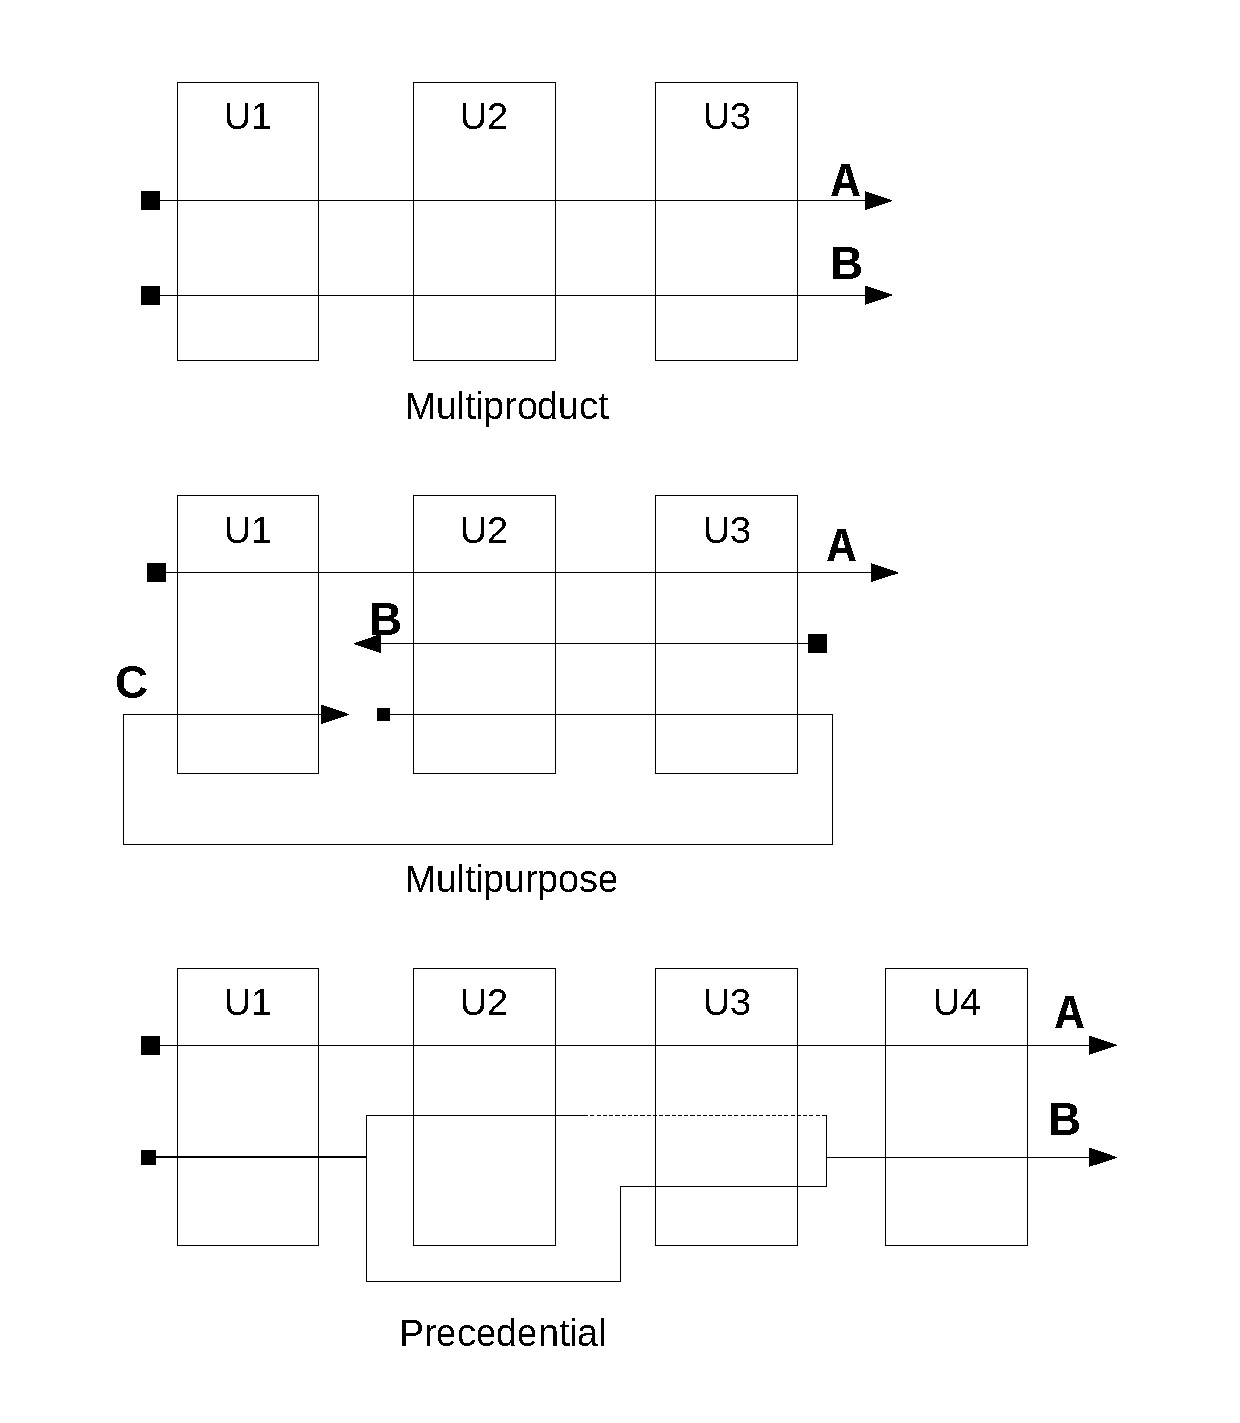
\includegraphics[scale=0.5]{receptek_block}
\caption{Különböző receptek szemléltetése blokkdiagramon}
\label{receptek_block}
\end{center}
\end{figure}

\newpage
A vegyipari, gyártási ütemezési feladatoknál nagy szerepet játszik a tárolási irányelv, amely azt mutatja meg, hogy két egymást követő feladat között az elkészített köztes termékeket hogyan kell raktározni, tárolni, illetve ez mennyi ideig lehetséges.
A tárolási irányelvek csoportosítására többféle lehetőség van.
Egyik dimenzió ezek közül, amikor az adott létesítmény infrastrukturális képességei korlátozzák az anyag mennyiségét és tárolásának módját.
\begin{itemize}
	\item \textbf{UIS - Unlimited Intermediate Storage}
	\item \textbf{FIS - Finite Intermediate Storage}
	\item \textbf{NIS - No Intermediate Storage}
\end{itemize}

Az UIS eset a legmegengedőbb.
Ebben az esetben van lehetőség a köztes anyagok bármely mértékű tárolására.
FIS esetben van lehetőség a tárolásra, de csak korlátozott mennyiségben.
A NIS esetében nincs külön tárolásra alkalmas egység, de az megoldható, hogy amíg a következő feldolgozó egységhez kerül, addig az előző taszk feldolgozó egységében várakozzon.	

A tárolás másik dimenziójának alapját az idő adja, amely a köztes termék kémiai és fizikai tulajdonságait befolyásolhatja.
Például a termék szavatossága, hőmérséklete megfelelő maradjon a következő részfeladat elkezdéséig.	
\begin{itemize}
	\item \textbf{UW - Unlimited Wait}
	\item \textbf{LW - Limited Wait}
	\item \textbf{ZW - Zero Wait}	
\end{itemize}

ZW esetben nincs lehetőség a köztes anyag tárolására, azaz ha a berendezés befejezte a munkát, akkor azonnal folytatni kell a gyártást.
Az LW esetben van egy idő, amíg a köztes termék várakozhat.
Azonban, ha ez a rendelkezésre álló idő elfogy, akkor muszáj folytatni a gyártás folyamatát.
Az UW eset a legmegengedőbb mind közül, ugyanis ha a köztes anyag tulajdonságai lehetőséget biztosítanak, akkor a tárolási idő nincs korlátozva, bármennyi ideig lehetőség van a tárolásra, raktározásra.

\section{Megoldó módszerek az irodalomban}
Az ütemezési feladatok megoldására számos megoldó módszer létezik.
Ezek közül a legismertebbek, és legszélesebb körben elterjedt módszerek kerülnek bemutatásra a dolgozatom következő pontjaiban.

\subsection{MILP modellek}
Az egyik legszélesebb körben elterjedt modell a \textbf{M}ixed \textbf{I}nteger \textbf{L}inear \textbf{P}rogramming \cite{Mendez2006} \cite{Floudas2004}, azaz a vegyes egészértékű lineáris programozás.
Az ilyen modellekben vegyesen fordulnak elő folytonos és egész változók. Többféle csoportba sorolhatók a modellek:
\begin{itemize}
  \item[] \textbf{Időfelosztásos modellek - Time discretization based models:}
  A módszer időpontokat és időréseket határoz meg.
  Időrendben az ilyen típusú készítmények jelentek meg először az irodalomban \cite{kondili}.
  Az időrésen és az időponton alapuló megközelítések sok hasonlóságot mutatnak, mivel egy időintervallumot, ami egy adott időponttól a következő időpontig tart, tekinthetünk egy időrésnek \cite{susarla}.
  Ellenkező irányból nézve pedig egy időrés kezdő időpontját egy időpontnak tekinthetjük.  
  
Minden időpontban bináris változók vannak hozzárendelve a feladatokhoz aszerint, hogy az adott időpillanatban elkezdődik a feladat végrehajtása vagy sem.
A bináris változók száma arányos lesz a kiválasztott időpontok számával, ezért a megoldáshoz szükséges idő nagy mértékben függ az időpontok számától.
Mindig megvolt a szándék olyan módszer kifejlesztésére, amelyben a szükséges időpontok száma minél kisebb legyen amellett, hogy megtalálja az optimális megoldást.
Létrejöttek jobb modellek, azonban készültek olyanok is, amelyek kevésbé voltak átláthatóak, a korlátozások még bonyolultabbá váltak, és modellezési hibák is előfordultak.
  
  \item[] \textbf{Precedencia alapú modellek - Precedence based models:}
  Az időfelosztásos módszerekkel szemben, ezeknél a módszereknél nincs szükség az időhorizont diszkretizációjára, azaz nem használnak ismeretlen paramétert a modellben.
  Az általuk kezelt problémákra általánosságban jobb számítási eredményeket nyújtanak, azonban ez a készlet sokkal kisebb, mint az időfelosztásos modellekhez tartozó kollekció.
  Alapvetően a multiproduct és multipurpose receptek esetében használható megfelelően, de kibővíthető, hogy a sokkal általánosabb precedential receptek is megoldhatók legyenek ezek segítségével. 
  
Ez a módszer kétféle bináris változót használ.
Az első $Y_{i,j}$, aminek az értéke abban az esetben lesz 1, ha $i$ feladatot $j$ berendezés végzi el.
A második változó: $X_{i,j,i'}$.
Értéke akkor lesz 1, ha ugyanaz a $j$ berendezés végzi el az $i$ és $i'$ taszkot, méghozzá úgy, hogy előbb az $i$-t teljesíti. 
\end{itemize}

\subsection{Analízis alapú eszközök}
Az automatákat és Petri hálókat széles körben alkalmazzák diszkrét eseményű rendszerek modellezésére \cite{cassandras}.
Számos kísérletet tettek ezen eszközök modellezési teljesítményének kiterjesztésére annak érdekében, hogy batch folyamatok ütemezésére is alkalmassá tegyék az említett eszközöket.
A meglévő modelleket időzítéssel egészítették ki, így jöttek létre a Timed Place Petri Nets (TPPN) and Timed Priced Automata (TPA) módszerek, amelyek Branch and Bound algoritmust használnak azért, hogy a legelőnyösebb megoldást megtalálják.
Ezen módszereknek a hatékonysága elmarad a MILP és az S-gráf modell hatékonyságától is.
\begin{itemize}
	\item[] \textbf{Időzített automaták:}
	Ezekben a megközelítésekben a recepteket és a berendezéseket külön modellezik, és ezeknek a párhuzamos összetételével jön létre a rendszer modellje.
	A bonyolultságot az jelenti, hogy az órák állapota végtelen lehet, és emiatt a rendszer állapotterülete is az lehet.
	\item[] \textbf{Időzített Petri háló:}
	Az alap ilyen módszereknél, hogy az átvitel jele késleltetés alapján jön létre.
	Többen is foglalkoztak a témával, például Ghaeli \cite{ghaeli}, aki batch folyamatok ütemezésével tanulmányozta.
\end{itemize}

\section{S-gráf módszertan}
Az S-gráf keretrendszer volt az első olyan publikált módszer, amely gráf elméleten alapult, valamint szakaszos gyártórendszerek ütemezési problémáinak megoldására szolgált \cite{combtech}.
Ez a keretrendszer egy irányított gráf modellből, az S-gráfból, és a hozzá tartozó algoritmusokból áll \cite{combframe}.
Az S-gráf egy speciális irányított gráf, amely ütemezési problémák számára lett létrehozva.
Nemcsak a recept vizualizációja, hanem egyben matematikai modell is.
A keretrendszerben az S-gráf reprezentálja a recepteket, a részleges és a teljes ütemterveket is.
Ezekben a gráfokban a termékeket és a feladatokat csúcsok jelölik, amelyeket csomópontoknak (node) nevezünk.
Az ütemezési döntés nélküli S-gráfot \textbf{Receptgráfnak} nevezzük.
Erre példa a~\ref{receptGraf} ábrán látható \cite{Hegyhati}. 
\begin{figure}[H]	
\begin{center}
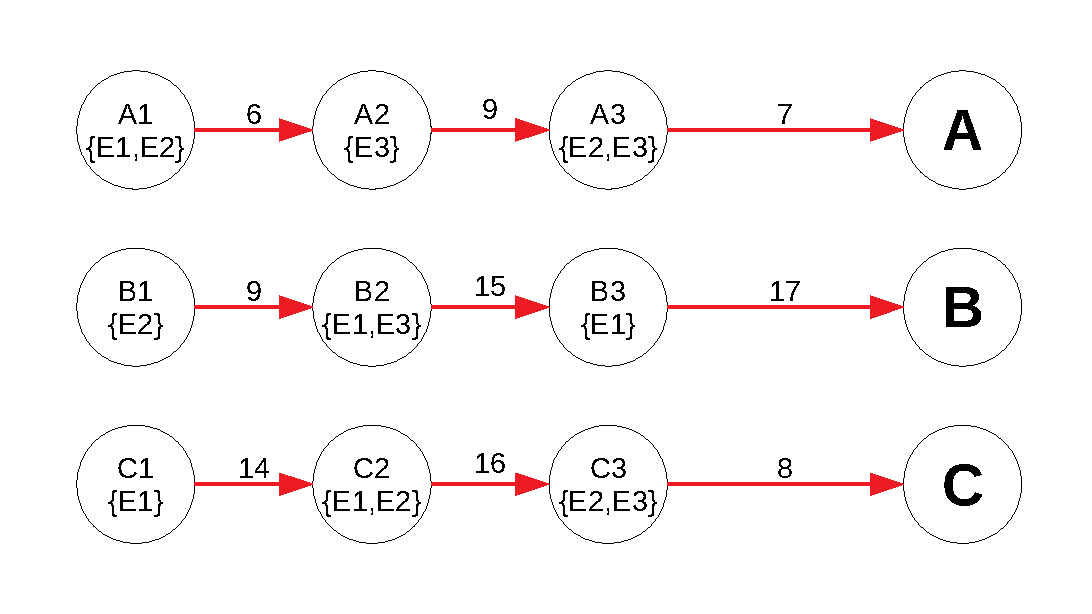
\includegraphics[scale=0.7]{receptGraf}
\caption{A receptgráf szemléltetése}
\label{receptGraf}
\end{center}
\end{figure}

A jobb oldalon látható három, nagybetűvel jelölt csomópont felel meg a termékeknek, a maradék kilenc pedig a részfeladatokat jelenti.
A részfeladatokon fel van tüntetve azon berendezések halmaza, amelyek az adott feladatot el tudják végezni.
Ezt a kilenc részfeladatot el kell végezni a termékek előállításának érdekében.
Az élek a csomópontok közti függőséget mutatják meg.
Ezeket \textbf{Receptéleknek} nevezzük.
Kétfajta függőséget tudunk megkülönböztetni:
\begin{itemize}
  \item Két részfeladat között van él.
  Ebben az esetben az egyik készíti el a másiknak a bemenetét.
  \item Egy termék és egy részfeladat között szerepel él.
  Ilyenkor a részfeladat készíti el a terméket.
\end{itemize}
Az éleken látható súlyok a részfeladat végrehajtásához szükséges időt mutatják meg.
Ha egy részfeladatot több berendezés is képes elvégezni, akkor az előbb említett súly mindig a legkisebb előállítási idő lesz.

Minden S-gráfhoz kapcsolódó algoritmus kiegészíti ezeket a gráfokat az úgynevezett \textbf{ütemezési élekkel}, amelyek az ütemezési döntést testesítik meg.
Ezekkel az élekkel kiegészített gráfoknak a neve \textbf{Ütemezési gráf}.
Példa a~\ref{utemezesiGraf} ábrán nézhető meg.
Az ábrán sötétkékkel jelölt élek az ütemezési élek.
Az ütemezési élek súlya alapértelmezetten nulla, ha a probléma nem tartalmaz szállítási, vagy tisztítási időt.
A részfeladatok csomópontjain már nem a lehetséges berendezések halmaza látható, hanem egy konkrét kiválasztott berendezés, az ütemezési döntésnek megfelelően. 
\begin{figure}[H]
\begin{center}
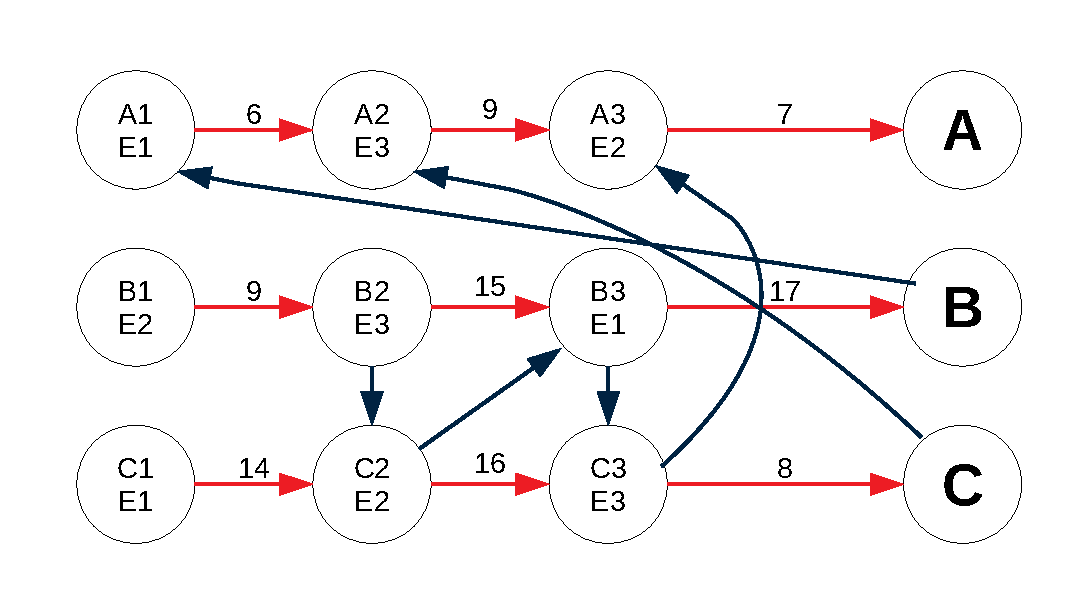
\includegraphics[scale=0.7]{utemezesiGraf}
\caption{Az ütemezési gráf szemléltetése}
\label{utemezesiGraf}
\end{center}
\end{figure}

Ugyanahhoz a berendezéshez rendelt részfeladatok végrehajtási sorrendje könnyedén leolvasható a gráfról.
A~\ref{utemezesiGraf2} ábrán látható példában az E2-es berendezés által elvégzett részfeladatok sorrendje B1 $\to$ C2 $\to$ A3.
Az ütemezési él azt mutatja meg, hogy nem elég az, hogy az E2 berendezés végrehajtsa a B1 feladatot, hanem ezt a közbenső terméket a B2 feladathoz tartozó E3 berendezés átvegye.
Csak ezeket követően tudja megkezdeni az adott részfeladat végrehajtását.
\begin{figure}[H]
\begin{center}
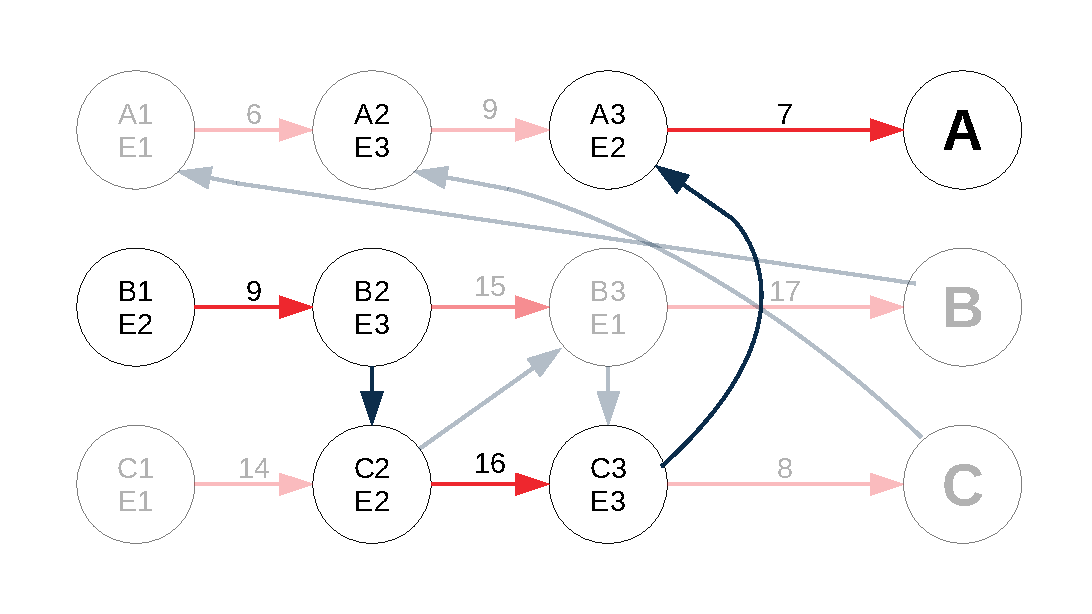
\includegraphics[scale=0.7]{utemezesiGraf2}
\caption{E2-es berendezés által elvégzett részfeladatok}
\label{utemezesiGraf2}
\end{center}
\end{figure}

Gyakran használt mód az ütemezési feladatok ábrázolására a Gantt diagram\cite{ganttwwf}, \cite{ganttofw}.
Ezeken a diagramokon a függőleges tengelyen a berendezések, míg a vízszintes tengelyen pedig az idő szerepel.
Az ábrán látható erőforrások szemléltetik az erőforrások elfoglaltságát.
Egy Gantt diagram látható a~\ref{GanttDiagram} ábrán.
\begin{figure}[H]
\begin{center}
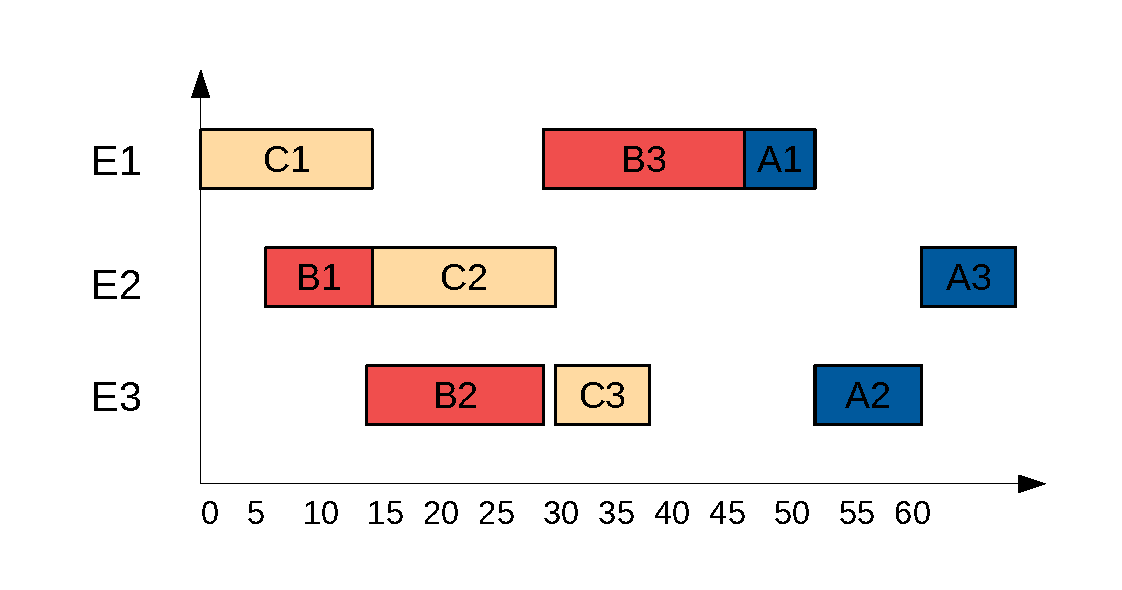
\includegraphics[scale=0.7]{GanttDiagram}
\caption{Egy ütemezés Gantt diagramon való megjelenítése}
\label{GanttDiagram}
\end{center}
\end{figure}

\subsection{A makespan minimalizálás algoritmusa}
Az egyik legelső célja az S-gráf keretrendszer létrehozásának a makespan minimalizálás volt.
Ennek alapja egy Branch \& Bound algoritmus, amivel lehetséges a termékek előállítási idejét minimalizálni.

Az algoritmus első lépésben inicializálja a $makespan^{cb}$ értékét végtelennel, majd az $S$ halmazt beállítja, amelyben az ütemezés során a nyitott részproblémák szerepelnek.
Csak a gyökér probléma szerepel benne kezdetben, vagyis egy receptgráf bármilyen hozzárendelés nélkül.
A \textbf{recipe} függvény visszaadja a probléma receptgráfjának modelljét, amit a $G(N,A_1,A_2,w)$ jelöl, amiben:
\begin{itemize}
	\item $N:$ a csomópontok halmaza (termékek és taszkok együttese)
	\item $A_{1}:$ a receptélek halmaza
	\item $A_{2}:$ az ütemezési élek halmaza (itt még üres halmaz)
	\item $w_{i,i^{'}}:$ a receptélekhez tartozó súlyok, amelyek az $i$ taszkok feldolgozási idejét jelentik.
	Kezdetben ez a legkisebb feldolgozási idő.
\end{itemize}

Az iteráció minden lépésében egy tetszőleges részprobléma kerül kiválasztásra a \textbf{select\_remove} függvénnyel, majd az $S$-ből eltávolításra.
Ennek a függvénynek a viselkedése a különböző megvalósításokban más és más lehet, ami más keresési stratégiát eredményez.
A kiválasztott részprobléma a következőképpen néz ki $(G(N,A_1,A_2,w),I',J',{\cal A})$, ahol:
\begin{itemize}
	\item $G(N,A_{1},A_{2},w):$ az ütemezési gráf
	\item $I^{'}:$ a még nem ütemezett taszkok halmaza
	\item $J^{'}:$ azon berendezések halmaza, amelyekhez az algoritmus még tud rendelni taszkokat 
	\item $\cal{A}:$ taszk-berendezés hozzárendelések halmaza, $(i,j)$ párok formájában 
\end{itemize}

Az iteráció elején kiértékelődik, hogy a részprobléma képes-e egy optimális megoldást nyújtani vagy sem.
Ez a \textbf{bound} függvénnyel történik.
Ezzel szemben több követelmény áll fenn.
Alsó korlátot kell adnia azoknak a megoldásoknak, amelyek a részproblémából származnak.
Biztosítania kell levél problémák pontos makespanjét.
Végtelen értékkel térjen vissza, ha a gráf tartalmaz kört, és jelezze, hogy megoldhatatlan.
A leggyakrabban a leghosszabb út keresésével vizsgálja meg a részproblémát a \textbf{bound} függvény, de lehetséges LP alapú modellek használata is.

Ha a korlát nem kisebb, mint az eddig megtalált legjobb eredmény, akkor az iteráció véget ér, és amennyiben létezik egy következő részprobléma, akkor az kerül kiválasztásra.
Ha viszont kisebb a korlát, abban az esetben ellenőrzi az algoritmus azt, hogy az összes taszk már ütemezett-e, vagyis a még nem ütemezett taszkok halmaza üres már ($I^{'}=\emptyset$).
Ha így van frissül a legjobb megoldás gráfja, a legjobb makespan és a hozzárendelések halmaza.
Ellenben, ha még szükséges további ütemezés, akkor a \textbf{select} függvény kiválaszt egy rendelkezésre álló berendezést a $J^{'}$ halmazból.
A kiválasztott $j$ berendezéshez az algoritmus hozzárendeli az összes lehetséges taszkot, mindegyiket külön-külön gyerekként, a még nem ütemezett taszkok és a kiválasztott berendezés által elvégezhető taszkok közös halmazából ($i \in I_{j} \cap I^{'}$).
Ezek a kiválasztott taszkok kapnak egy másolatot az aktuális S-gráfról.
Mivel a csomópontok és a receptélek halmaza nem változik, ezért ezek változatlanok maradnak, csak az ütemezési élek halmaza és súlyok változnak.
Ezt a másolatot kibővíti az algoritmus az új hozzárendelés alapján az ütemezési élekkel ($A^{i}_{2}:= A^{i}_{2} \cup \{(i^{'},i)\}$).
Ezután minden $i$-ből induló receptél súlya frissül a $t^{pr}_{i,j}$ értékével.
Végezetül pedig az új részproblémát hozzáadja az $S$ halmazhoz.
Itt $I^{'}$ halmazból kikerül az előbb kiválasztott $i$ taszk, és a hozzárendelések halmazába bekerül az új taszk-berendezés pár (${\cal A}\cup\{(i,j)\}$).

Abban az esetben, ha minden még nem ütemezett taszkot a kiválasztott $j$ berendezésen kívül más berendezés is el tud végezni, akkor egy új részproblémát hoz létre az algoritmus, amelyben a $j$ berendezés már nem végez több taszkot, azaz kikerül a még rendelkezésre álló berendezések halmazából ($J^{'}\setminus\{j\}$).

Ha az $S$ halmaz üres lesz, akkor a $G^{cb}$ gráf és a hozzárendelések a ${\cal A}^{cb}$ halmazban leírják az optimális megoldást.
Ha legalább egy megvalósítható, akkor az algoritmus visszatér ezzel az értékkel, ellenkező esetben nem ad vissza megoldást.

\begin{algorithm}[H]
\caption{A makespan minimalizálás pszeudó kódja}
\label{makespan_min}
\begin{algorithmic}[1]
  \State $makespan^{cb}:= \infty$
  \State ${\cal S}:= \{($\textbf{recipe()}$,I,J,\emptyset)\}$  
  \While {${\cal S}\ne\emptyset $}
    \State $(G(N,A_1,A_2,w),I',J',{\cal A}):= $\textbf{select\_remove(}$\cal S$\textbf{)}
    \If{\textbf{bound(}$G$\textbf{)}$<makespan^{cb}$}
      \If{$I'=\emptyset$}
        \State $makespan^{cb}:= $\textbf{bound(}$G$\textbf{)}
        \State $G^{cb}\:= G$
        \State ${\cal A}^{cb}:= {\cal A}$        
      \Else
        \State $j:= $\textbf{select(}$J'${)} 
        \ForAll{$i \in I_j \cap I'$}
          \State $G^i(N,A_1,A^i_2,w^i):= G(N,A_1,A_2,w)$
          \ForAll{$i' \in \bigcup_{(i',j)\in{\cal A}}I^+_{i'}\setminus\{i\}$}
            \State $A^i_2:= A^i_2 \cup \{(i',i)\}$
          \EndFor        
          \ForAll{$i' \in I^+_{i}$}
            \State $w^i_{i,i'}:= t^{pr}_{i,j}$
          \EndFor
          \State ${\cal S}:= {\cal S} \cup (G^i(N,A_1,A^i_2,w^i),I'\setminus\{i\},J',{\cal A}\cup\{(i,j)\})$
        \EndFor
        \If{$I'\subseteq\bigcup_{j'\in J',j\ne j'}I_{j'}$}
          \State ${\cal S}:= {\cal S} \cup (G(N,A_1,A_2),I',J'\setminus\{j\},{\cal A})$
        \EndIf
      \EndIf %ha nem megoldas 
    \EndIf % bound jo
  \EndWhile % S minden elemere
  \If {$makespan^{cb}\ne\infty$}
    \State \textbf{return} ($G^{cb},{\cal A}^{cb}$)
  \EndIf
\end{algorithmic}
\end{algorithm}

\newpage
\subsection{Throughput maximalizálás}
Eredetileg az S-gráf keretrendszer makespan minimalizációs problémák megoldására lett létrehozva, azonban a későbbiekben bővítésre került, így ezután throughput, profitmaximalizációs problémák megoldására is alkalmazhatóvá vált.
Az alapötlet Majozi és Friedler \cite{majozifriedler}, valamint Holczinger és társai \cite{holczinger} nevéhez fűződik.
A termékek lehetséges batch darabszámai alapján az algoritmus konfigurációkat hoz létre.
A konfiguráció tehát az, ami megmutatja, hogy egy termékből hány batch készül el.
Ha $n$ a termékek számát jelöli, akkor egy $n$ dimenziós térben lehet elképzelni ezeket a konfigurációkat. 

\begin{algorithm}[H]
\caption{Az algoritmus pszeudó kódja}
\label{throughput}
\begin{algorithmic}[1]
  \State $revenue^{cb}:=  0$
  \State ${\cal S}:=  (\mathbb{Z}^*)^{|P|}$
  \While {${\cal S}\ne\emptyset$}
    \State $x:= $\textbf{select\_remove(}$\cal S$\textbf{)}
    \If{\textbf{feasible(recipe(}$x$\textbf{),$t^H$)}}
      \If{\textbf{revenue(}$x$\textbf{)}$>revenue^{cb}$}
        \State $revenue^{cb}:= $\textbf{revenue(}$x$\textbf{)}
        \State $x^{cb}:=  x$
        \State \textbf{update(}${\cal S},revenue^{cb}$\textbf{)}
      \EndIf
    \Else
      \State ${\cal S}:= \{ x'\in{\cal S} \mid x' \not\ge x\}$
    \EndIf
  \EndWhile
  \If {$revenue^{cb}\ne 0$}
    \State \textbf{return} ($x^{cb},revenue^{cb}$)
  \EndIf
\end{algorithmic}
\end{algorithm}

Az algoritmus először inicializálja az $S$ halmazt a termékekre vonatkozóan minden lehetséges batch számmal.
Fontos kiemelni, hogy ebben az esetben minden terméknél a batch méret rögzített, azaz egy termék batch-jének jövedelme ismert.
Ezt követően minden iteráció során az előbb említett halmazból kiválasztásra kerül egy konfiguráció a \textbf{select\textunderscore remove} függvény segítségével.
Ezután sor kerül a megvalósíthatóság tesztelésére, amely során eldől, hogy a megadott időhorizont alatt megvalósítható vagy sem.
Ha megvalósítható és nagyobb jövedelmet biztosít, mint az eddig megtalált legnagyobb jövedelem, akkor a jelenlegi legjobb megoldás és az S halmaz frissül.
Ha infeasible a kiválasztott konfiguráció, akkor ez, és minden ennél nagyobb konfiguráció eltávolításra kerül az S halmazból.
Amint az S halmaz üressé válik, és volt feasible megoldás, akkor az algoritmus visszatér a legjobb konfigurációval, és az ehhez tartozó jövedelem mennyiségével.

A~\ref{throughput1} ábrán látható egy általam elkészített, Throughput módszerrel megvalósított feladat eredménye.
\begin{figure}[H]
\begin{center}
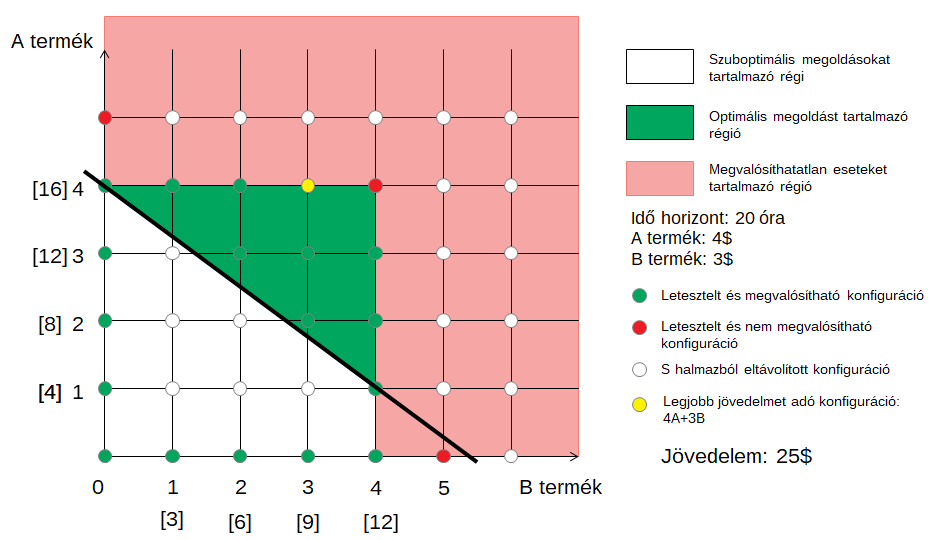
\includegraphics[scale=0.8]{throughput}
\caption{Throughput maximalizálás szemléltetés}
\label{throughput1}
\end{center}
\end{figure}

Két termék esetén koordináta rendszeren szemléltethető az algoritmus működése.
Egyik tengelyen az egyik termék, a másikon pedig a másik termék szerepel.
Kezdetben az összes konfigurációt tartalmazta a konfigurációk halmaza.
Az algoritmus először végighaladt az egyik tengely mentén, vagyis az egyik termék batch mérete 0 volt, a másik pedig növekedett.
Ezt a haladási irányt addig követte amíg megtalálta az első nem megvalósítható, azaz infeasible konfigurációt.
Ezt követően elvégzi a keresést a másik tengelyen is.
Így kapott egy jelenleg maximális jövedelmet.
Az utolsó még feasible batch számoknál nagyobb batch számokat már nem kell vizsgálni, hiszen azokat a megadott időhorizonton belül nem lehet megvalósítani.
A képen látható feladatban a legnagyobb elérhető profit 16 volt, amikor csak egy termék vizsgálata történt.
A feketével jelzett egyenesen szerepel az összes 16 profittal rendelkező pont.
Ezt az egyenest nevezzük revenue line-nak.
A B termékhez tartozó 16-os profitérték nem egész batch számhoz tartozik, a legközelebbi 15 profittal rendelkezik, ami infeasible már.
Az egyenes alatt azok a konfigurációk szerepelnek, amelyek jövedelme nem éri el a jelenlegi maximumot, így ezek nem a lehető legjobb megoldást adják meg.
Az algoritmus addig nem állt le, amíg a halmaz, amely a konfigurációkat tartalmazza ki nem ürül.
A példafeladatban a maximálisan elérhető jövedelem 25 egység.
Ezt 4 darab A termék és 3 darab B termék legyártásával lehet elérni.